\newpage

\subsection{Polygon triangulation}

\paragraph{Disposition}

\begin{itemize}
  \item hello, intro, and motivation.
  \item triangulation and monotonicity.
  \item algorithms and their complexities.
  \item proof: MAKE\_MONOTONE.
  \item proof: size of monotone decomposition.
\end{itemize}

\paragraph{Notes}

\begin{enumerate}
  \item hello.
  \item motivation: computer graphics, computational geometry.

  \item describe triangulation and (y-)monotonicity.

  \item $n := |V|$.

  \item TRIANGULATE\_MONOTONE\_POLYGON in $O(n)$ time.
  \item MAKE\_MONOTONE in $O(n \lg n)$ time.

  \item show MAKE\_MONOTONE partitions $P$ into monotone subpolygons \\(for
    HANDLE\_SPLIT\_VERTEX only) with only legal diagonals.
  \item show size of monotone decomposition is $O(n)$.
\end{enumerate}

\begin{figure}[H]
  \centering
  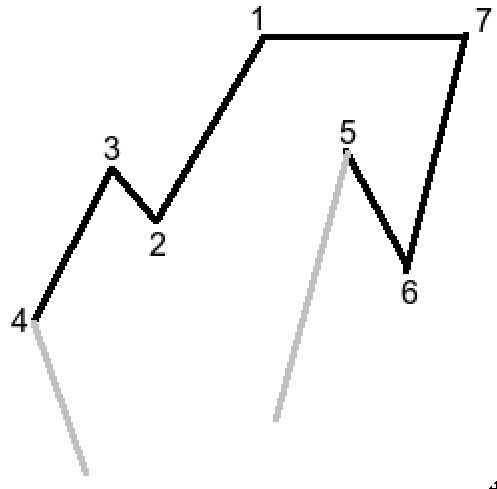
\includegraphics[width=0.5\textwidth]{figures/monotonization_example.png}
  \caption{Polygon monotonization example.}
  \label{fig:monotonization_example}
\end{figure}
